\documentclass[aps,prb,reprint,superscriptaddress,longbibliography]{revtex4-2}

\usepackage{amsmath,amssymb}
\usepackage{bm}
\usepackage{booktabs}
\usepackage{graphicx}
\usepackage[colorlinks=true,citecolor=blue,urlcolor=blue,linkcolor=blue]{hyperref}

\newtheorem{theorem}{Theorem}
\newcommand{\ENa}{E_{N,a}}
\newcommand{\Ehat}{\widehat E}

\begin{document}

\title{Two-scale finite-size edge splitting at a repeated root of an extended Su--Schrieffer--Heeger chain}

\author{Xiaojian Zeng}
\email{xiaojianzeng@foxmail.com}
\affiliation{PBC School of Finance, Tsinghua University, Beijing 100190, China}

\date{September 14, 2026}

\begin{abstract}
Repeated decay roots in a finite topological chain produce power-law-prefactored
edge profiles, but the collision of the usual root vectors makes a direct
finite-chain projection singular.  We resolve this collision for the open
extended Su--Schrieffer--Heeger family with hoppings
$u_0=r^2$, $u_1=2r$, and $u_2=1$.  A root-and-derivative boundary basis gives
two positive projected energies in closed form.  More importantly, a signed
reversal maps the rescaled inverse hopping block to a rank-two matrix plus an
explicit triangular tail.  Singular-value perturbation then gives a uniform
relative enclosure for every $r\in[1/5,4/5]$ and integer $N\geq61$.
The two exact positive edge energies satisfy
\begin{equation*}
 E_{N,1}\sim \frac{(1-r^2)r^{N+1}}{N},\qquad
 E_{N,2}\sim N(1-r^2)^3r^{N-1},
\end{equation*}
uniformly on this interval.  A min--max estimate places the third positive
energy at or above the bulk-band distance $(1-r)^2$, proving that precisely
four chiral in-gap levels occur in the certified range.  Thus a single
double bulk root produces two parametrically different finite-size
hybridization scales rather than one common exponential splitting.
\end{abstract}

\maketitle

\section{Introduction}

The Su--Schrieffer--Heeger (SSH) chain was introduced as a model of
polyacetylene \cite{Su1979} and is now a canonical setting in which chiral
symmetry relates a bulk winding number to boundary-localized states
\cite{Grizzi2026}.  Longer-range intersublattice hopping extends the winding
number beyond unity and permits several boundary pairs.  Such extended SSH
(eSSH) structures have been studied dynamically \cite{Ghosh2023} and realized
in long-range-coupled photonic lattices \cite{Li2024}.  For a finite device,
the nominally zero-energy states at opposite ends hybridize.  Their small
energies, rather than the semi-infinite zero modes alone, determine whether
the edge multiplet can be spectrally resolved.

Generalized Bloch theory provides exact bulk and boundary equations for
finite-range free-fermion Hamiltonians \cite{Alase2016,Alase2017}.  When a
transfer or decay root is defective, its boundary profile acquires a
power-law prefactor.  This general mechanism is known and is not the subject
of the present work.  A recent analysis of the eSSH model derived exact
semi-infinite edge states and accurate finite-chain expressions for two
distinct complex-conjugate roots \cite{Grizzi2026}.  On the discriminant line
where the two roots coincide, however, those two root vectors become
linearly dependent.  The finite-chain overlap matrix in the distinct-root
representation is then singular, even though the physical two-dimensional
edge space remains well defined through a confluent root-and-derivative
basis.

Here we solve the finite-size splitting on one such repeated-root line.  The
model is simple enough that its off-diagonal block is
$T_N=(rI+S_N)^2$, but the two smallest singular values occur at different
polynomial orders in $N$.  We first construct the exact four-state confluent
Gram pencil.  We then convert $r^{N+1}T_N^{-1}$, by orthogonal sign and reversal
operations, into a symmetric rank-two matrix plus a triangular tail whose
Frobenius norm is an explicit finite sum.  This supplies a relative enclosure,
not merely a residual estimate.  General Toeplitz finite-section theory
already gives qualitative splitting results \cite{Rogozhin2006}; the result
below is the pair of coefficients, an explicit uniform remainder, and the
exact in-gap count for this fixed Hermitian family.

\section{Open repeated-root chain}
\label{sec:model}

Let $N\geq3$ be the number of unit cells, with orthonormal orbitals
$\{|A_j\rangle,|B_j\rangle\}_{j=0}^{N-1}$.  We set the long hopping $u_2=1$
as the energy unit and take
\begin{equation}
 u_0=r^2,\qquad u_1=2r,\qquad r\in I:=[1/5,4/5].
\end{equation}
The open, single-particle Hamiltonian is
\begin{align}
 H_N={}&\sum_{j=0}^{N-1}r^2|B_j\rangle\langle A_j|
 +\sum_{j=0}^{N-2}2r|B_j\rangle\langle A_{j+1}| \nonumber\\
 &+\sum_{j=0}^{N-3}|B_j\rangle\langle A_{j+2}|+\mathrm{H.c.}
 \label{eq:H}
\end{align}
There are no on-site or wrap-around terms.  In the $A$-then-$B$ basis,
\begin{equation}
 H_N=\begin{pmatrix}0&T_N^T\\T_N&0\end{pmatrix},\qquad
 T_N=r^2I+2rS+S^2=(rI+S)^2,
 \label{eq:block}
\end{equation}
where $S_{jk}=\delta_{k,j+1}$.  Hence $H_N$ is real, Hermitian, and chiral.
Writing the singular values of $T_N$ as
$0<E_{N,1}\leq\cdots\leq E_{N,N}$, the spectrum of $H_N$ consists of
$\{\pm E_{N,a}\}_{a=1}^N$.

For $z=e^{-ik}$, the periodic off-diagonal symbol is
\begin{equation}
 Q_1(z)=r^2+2rz+z^2=(z+r)^2.
 \label{eq:symbol}
\end{equation}
The root $z=-r$ has multiplicity two and lies strictly inside the unit disk.
With the convention of Ref.~\cite{Grizzi2026}, the winding number is two.
The distance from zero to either periodic bulk band is
\begin{equation}
 \Delta_g(r)=\min_{|z|=1}|Q_1(z)|=(1-r)^2\geq\frac1{25}.
 \label{eq:bulkgap}
\end{equation}
We use ``in-gap'' below to mean $|E|<\Delta_g$; the full interband gap is
$2\Delta_g$.

\section{Collision-safe four-state pencil}
\label{sec:pencil}

Put $q=r^2$ and $z=-r$.  On the left edge define the two real vectors
\begin{equation}
 u_i=z^i,\qquad w_i=i z^{i-1},\qquad i=0,\ldots,N-1,
 \label{eq:uw}
\end{equation}
with $w_0=0$.  They are the root and derivative profiles at the double root.
Let $R$ reverse the cell order, $(Rx)_i=x_{N-1-i}$, and use $Ru,Rw$ on the
right edge.  In the ordered basis $(u,w,Ru,Rw)$, with the first pair on the
$A$ sublattice and the reflected pair on the $B$ sublattice, introduce
\begin{align}
 A_N&=\sum_{i=0}^{N-1}q^i,&
 B_N&=\sum_{i=0}^{N-1}i q^i,&
 D_N&=\sum_{i=0}^{N-1}i^2q^i,\nonumber\\
 \Delta_N&=A_ND_N-B_N^2.&&&
 \label{eq:sums}
\end{align}
Direct summation gives the exact Gram and projected Hamiltonian matrices
\begin{equation}
 G=\begin{pmatrix}G_L&0\\0&G_L\end{pmatrix},\quad
 G_L=\begin{pmatrix}A_N&-B_N/r\\-B_N/r&D_N/r^2\end{pmatrix},
 \label{eq:gram}
\end{equation}
\begin{equation}
 K=\begin{pmatrix}0&C\\C&0\end{pmatrix},\quad
 C=\begin{pmatrix}0&-z^N\\-z^N&-Nz^{N-1}\end{pmatrix}.
 \label{eq:cross}
\end{equation}
The cross block follows without an asymptotic truncation.  Indeed, the
double-root recurrence cancels all but the last two components:
\begin{align}
 T_Nu&=(0,\ldots,0,-z^N,z^{N+1})^T,\nonumber\\
 T_Nw&=(0,\ldots,0,-Nz^{N-1},(N-1)z^N)^T.
 \label{eq:boundaryres}
\end{align}
The finite sums in Eq.~\eqref{eq:sums} can be evaluated without cancellation
as sums, or in closed form as
\begin{align}
 A_N={}&\frac{1-q^N}{1-q},\nonumber\\
 B_N={}&\frac{q-Nq^N+(N-1)q^{N+1}}{(1-q)^2},\nonumber\\
 D_N={}&\frac{q(1+q)-N^2q^N}{(1-q)^3}\nonumber\\
 &+\frac{(2N^2-2N-1)q^{N+1}-(N-1)^2q^{N+2}}
 {(1-q)^3}.
 \label{eq:closedsums}
\end{align}

Define
\begin{equation}
 m_N=NA_N-2B_N,\qquad
 \phi_{1,N}=\frac{\sqrt{m_N^2+4\Delta_N}+m_N}{2},
 \label{eq:phi1}
\end{equation}
\begin{equation}
 \phi_{2,N}=\frac{\sqrt{m_N^2+4\Delta_N}-m_N}{2}
 =\frac{\Delta_N}{\phi_{1,N}}.
 \label{eq:phi2}
\end{equation}
For $N\geq61$, $m_N>0$ and
$\phi_{1,N}\geq\phi_{2,N}>0$.  Expanding
$\det(C-EG_L)$, or equivalently separating the two chiral parities of
$K\bm v=EG\bm v$, gives the two positive Ritz energies
\begin{equation}
 \boxed{
 \widehat E_{N,1}=\frac{r^{N+1}}{\phi_{1,N}},\qquad
 \widehat E_{N,2}=\frac{r^{N+1}}{\phi_{2,N}}.}
 \label{eq:ritz}
\end{equation}
Unlike a coincident-root substitution in a distinct-root basis,
Eqs.~\eqref{eq:gram}--\eqref{eq:ritz} retain the nonzero overlap $-B_N/r$
and remain nonsingular at the collision.

\section{Rank-two inverse comparison}
\label{sec:inverse}

The projected energies become controlled approximations to the exact
singular values because the full inverse has a nearly rank-two form.  Since
$S^N=0$,
\begin{equation}
 T_N^{-1}=\sum_{d=0}^{N-1}(-1)^d(d+1)r^{-d-2}S^d.
 \label{eq:inverse}
\end{equation}
A column reversal and diagonal sign changes preserve singular values and
map $r^{N+1}T_N^{-1}$ to the real symmetric matrix
\begin{equation}
 (M_N)_{i\ell}=
 \begin{cases}
 (N-i-\ell)r^{i+\ell},&i+\ell\leq N-1,\\
 0,&i+\ell\geq N,
 \end{cases}
 \label{eq:M}
\end{equation}
for $0\leq i,\ell\leq N-1$.  With $a_i=r^i$ and $b_i=ir^i$, extend the
nonzero branch of Eq.~\eqref{eq:M} over the full square:
\begin{equation}
 F_N=Naa^T-ba^T-ab^T.
 \label{eq:F}
\end{equation}
This matrix has rank two.  On $\operatorname{span}\{a,b\}$ its nonzero
eigenvalues have sum $m_N$ and product $-\Delta_N$.  They are therefore
$\phi_{1,N}$ and $-\phi_{2,N}$, so the two nonzero singular values of $F_N$
are exactly $\phi_{1,N}$ and $\phi_{2,N}$.

The remainder $R_N=M_N-F_N$ is supported on the opposite triangle:
\begin{equation}
 (R_N)_{i\ell}=(i+\ell-N)r^{i+\ell}
 \quad\text{for }i+\ell\geq N+1.
 \label{eq:R}
\end{equation}
Consequently
\begin{align}
 \epsilon_N(r):=\|R_N\|_F
 &=\left[\sum_{t=1}^{N-2}(N-1-t)t^2r^{2N+2t}\right]^{1/2}
 \label{eq:epsilon}\\
 &\leq r^{N+1}
 \sqrt{\frac{(N-1)(1+r^2)}{(1-r^2)^3}}.
 \label{eq:epssimple}
\end{align}
Let $\mu_{1,N}\geq\mu_{2,N}$ be the two largest singular values of $M_N$.
Inverse singular-value ordering and Eq.~\eqref{eq:M} give
\begin{equation}
 \mu_{a,N}=\frac{r^{N+1}}{E_{N,a}},\qquad a=1,2.
 \label{eq:muE}
\end{equation}
Weyl's singular-value inequality applied to $M_N=F_N+R_N$ then yields
\begin{equation}
 |\mu_{a,N}-\phi_{a,N}|\leq\epsilon_N(r),\qquad a=1,2.
 \label{eq:weyl}
\end{equation}

\section{Uniform enclosure and asymptotics}
\label{sec:theorem}

We now state the finite-size result.  Every constant is explicit; the
threshold $N=61$ is sufficient and is not claimed to be optimal.

\begin{theorem}
For every $r\in[1/5,4/5]$ and integer $N\geq61$,
$\epsilon_N<\phi_{2,N}\leq\phi_{1,N}$ and, for $a=1,2$,
\begin{equation}
 |E_{N,a}-\widehat E_{N,a}|\leq
 R_a(N,r):=\widehat E_{N,a}
 \frac{\epsilon_N(r)}{\phi_{a,N}-\epsilon_N(r)}.
 \label{eq:absolute}
\end{equation}
Moreover,
\begin{equation}
 \frac{|E_{N,a}-\widehat E_{N,a}|}{E_{N,a}}
 \leq\frac{\epsilon_N(r)}{\phi_{a,N}}
 \leq\eta_N,
 \label{eq:relative}
\end{equation}
where
\begin{equation}
 \eta_N=150N\left(\frac45\right)^{N+1}
 \sqrt{\frac{(N-1)(41/25)}{(9/25)^3}}.
 \label{eq:eta}
\end{equation}
The four closest-to-zero eigenvalues of $H_N$ are exactly
$-E_{N,2},-E_{N,1},E_{N,1},E_{N,2}$ and lie strictly inside the bulk gap.
Uniformly in $r$,
\begin{align}
 E_{N,1}&=\frac{(1-r^2)r^{N+1}}{N}[1+o(1)],\nonumber\\
 E_{N,2}&=N(1-r^2)^3r^{N-1}[1+o(1)].
 \label{eq:asymptotic}
\end{align}
\end{theorem}

\noindent\textit{Proof.}\ 
The Gram determinant has the Cauchy--Binet expansion
\begin{equation}
 \Delta_N=\sum_{0\leq i<j\leq N-1}(j-i)^2q^{i+j}
 \geq q\geq\frac1{25}.
 \label{eq:CB}
\end{equation}
The geometric-series bounds
\begin{equation}
 A_N\leq\frac{25}{9},\qquad
 D_N\leq\frac{q(1+q)}{(1-q)^3}\leq\frac{16400}{729}
\end{equation}
and $B_N\leq q/(1-q)^2\leq400/81$ show first that
$m_N\geq N-800/81>0$.  They then imply, for $N\geq61$,
\begin{equation}
 \phi_{1,N}\leq m_N+\sqrt{\Delta_N}\leq6N,\qquad
 \phi_{2,N}=\frac{\Delta_N}{\phi_{1,N}}\geq\frac{1}{150N}.
 \label{eq:phibounds}
\end{equation}
Combining Eqs.~\eqref{eq:epssimple} and \eqref{eq:phibounds}, maximizing the
elementary factors at $r=4/5$, gives
$\epsilon_N/\phi_{2,N}\leq\eta_N$.  Both comparisons
\begin{equation}
 \eta_{61}^2<\left(\frac{413}{1000}\right)^2,
 \qquad
 \left(\frac{\eta_{N+1}}{\eta_N}\right)^2
 =\frac{16}{25}\frac{(N+1)^2}{N(N-1)}<1
 \label{eq:etaexact}
\end{equation}
are rational inequalities after squaring and cross multiplication.  Thus
$\epsilon_N<\phi_{2,N}\leq\phi_{1,N}$ throughout the stated domain.
Equation~\eqref{eq:weyl} gives
$\mu_{a,N}\geq\phi_{a,N}-\epsilon_N>0$.  Taking reciprocals in
Eq.~\eqref{eq:muE} proves Eq.~\eqref{eq:absolute}; dividing by the exact
energy instead gives Eq.~\eqref{eq:relative}.  Because $\eta_N\to0$
exponentially, the control is uniformly relative.

For the leading terms, the finite sums obey, uniformly on $I$,
\begin{align}
 A_N&=\frac1{1-q}+O(q^N),\nonumber\\
 B_N&=\frac{q}{(1-q)^2}+O(Nq^N),\nonumber\\
 \Delta_N&=\frac{q}{(1-q)^4}+O(N^2q^N).
 \label{eq:sumasy}
\end{align}
Equations~\eqref{eq:phi1} and \eqref{eq:phi2} therefore give
\begin{align}
 \phi_{1,N}&=\frac{N}{1-q}[1+O(N^{-1})],\nonumber\\
 \phi_{2,N}&=\frac{q}{N(1-q)^3}[1+O(N^{-1})].
 \label{eq:phiasy}
\end{align}
Substitution into Eq.~\eqref{eq:ritz}, followed by the relative enclosure,
proves Eq.~\eqref{eq:asymptotic}.

It remains to count the in-gap levels.  Extend $x\in\mathbb C^N$ by zero to
$\ell^2(\mathbb Z)$ and let $U$ be the bilateral shift.  On the codimension-two
subspace $x_0=x_1=0$, no left-boundary output is lost, and hence
\begin{equation}
 \|T_Nx\|=\|(rI+U)^2x\|
 \geq\min_{|\zeta|=1}|r+\zeta|^2\|x\|
 =(1-r)^2\|x\|.
 \label{eq:minmax}
\end{equation}
The singular-value min--max principle implies
$E_{N,3}\geq(1-r)^2$.  Conversely, Eqs.~\eqref{eq:muE},
\eqref{eq:phibounds}, and \eqref{eq:relative} give
\begin{equation}
 E_{N,2}\leq\frac{150Nr^{N+1}}{1-\eta_N}
 \leq\frac{150(61)(4/5)^{62}}{1-413/1000}
 <\frac1{25}\leq(1-r)^2.
 \label{eq:E2gap}
\end{equation}
The middle strict inequality is again an exact rational comparison.  The
right-hand side is maximal at $N=61$ because $N(4/5)^{N+1}$ decreases and
$1-\eta_N$ increases thereafter.  Thus exactly two positive singular values
lie below the bulk-band distance.  Chiral symmetry supplies their two
negative partners, completing the proof. \hfill$\square$

The two splittings are parametrically separated:
\begin{equation}
 \frac{E_{N,2}}{E_{N,1}}
 \sim\frac{N^2(1-r^2)^2}{r^2}.
 \label{eq:ratio}
\end{equation}
Accordingly, the inner doublet $\pm E_{N,1}$ is much more weakly hybridized
than the outer doublet $\pm E_{N,2}$ even though both descend from the same
double decay root.

\begin{figure*}[t]
 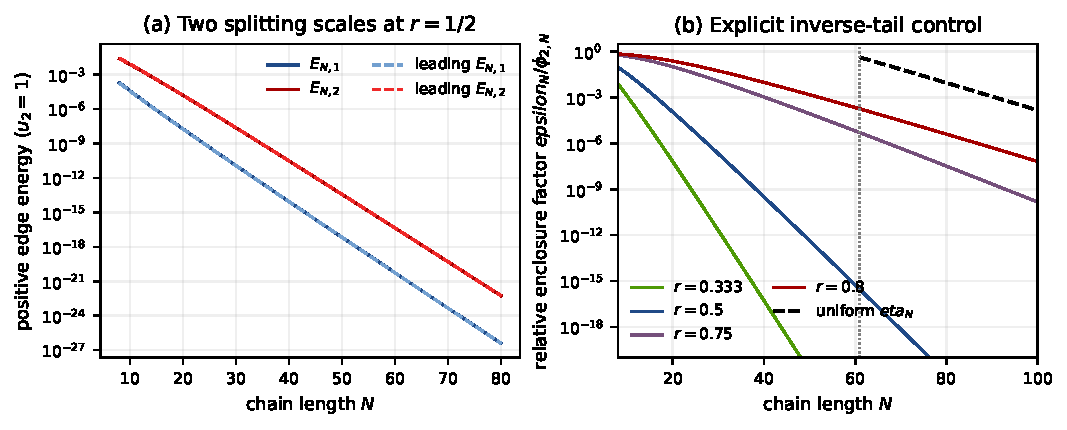
\includegraphics[width=\textwidth]{edge_splittings.pdf}
 \caption{Finite-size splitting and enclosure.  (a) The exact positive edge
 energies at $r=1/2$, evaluated stably from the two largest singular values
 of $M_N$, compared with the two leading laws in Eq.~\eqref{eq:asymptotic}.
 (b) The computable worst-branch factor $\epsilon_N/\phi_{2,N}$ for four
 values of $r$.  The dashed curve is the interval-uniform upper bound
 $\eta_N$, shown in its proven range $N\geq61$; the vertical dotted line marks
 the sufficient threshold.  The plotted points are direct evaluations of
 the displayed finite sums, with no fitted parameters.  The plotting code was
 generated with the AI assistance disclosed in Sec.~\ref{sec:numerics} and
 checked against the tabulated data and analytic expressions.}
 \label{fig:splitting}
\end{figure*}

\section{Numerical checks and reproducibility}
\label{sec:numerics}

Figure~\ref{fig:splitting}(a) evaluates the exact small singular values via
Eq.~\eqref{eq:muE}, avoiding loss of relative precision from a direct
double-precision diagonalization of $T_N^TT_N$.  Independent 110-decimal
diagonalization of $T_N^TT_N$ was also performed at
$r=1/3,1/2,3/4$ and $N=8,12,20,40$.  A separately assembled generalized
eigenproblem from Eqs.~\eqref{eq:gram} and \eqref{eq:cross} reproduced
Eq.~\eqref{eq:ritz}.  Table~\ref{tab:checks} reports the larger relative Ritz
error across the two positive branches.  These checks illustrate convergence
but are not used to infer the theorem.

\begin{table}[b]
\caption{Maximum relative Ritz error
$\max_{a=1,2}|E_{N,a}-\widehat E_{N,a}|/E_{N,a}$ from independent
high-precision diagonalization.}
\label{tab:checks}
\begin{ruledtabular}
\begin{tabular}{ccccc}
$r$ & $N=8$ & $N=12$ & $N=20$ & $N=40$\\
\colrule
$1/3$ & $9.73\!\times\!10^{-5}$ & $7.67\!\times\!10^{-8}$ & $1.35\!\times\!10^{-14}$ & $1.72\!\times\!10^{-32}$\\
$1/2$ & $1.16\!\times\!10^{-2}$ & $2.60\!\times\!10^{-4}$ & $3.20\!\times\!10^{-8}$ & $4.64\!\times\!10^{-19}$\\
$3/4$ & $2.97\!\times\!10^{-1}$ & $1.41\!\times\!10^{-1}$ & $1.33\!\times\!10^{-2}$ & $2.63\!\times\!10^{-6}$\\
\end{tabular}
\end{ruledtabular}
\end{table}

Exact-fraction tests independently checked the Gram block, cross-Hamiltonian
block, rescaled-inverse transformation, and tail norm in 40 cases obtained by
crossing $N=3,\ldots,10$ with
$r\in\{1/5,1/3,1/2,3/4,4/5\}$.  The accompanying reproducibility package
contains the high-precision validation program, the exact-fraction checker,
the figure-generation program, and the tabulated figure data.  The recorded
environment uses Python 3.12.14, NumPy 2.3.5, SciPy 1.18.1, mpmath 1.3.0, and
Matplotlib 3.11.2.

\smallskip\noindent\textit{AI-assisted research disclosure.}\ 
OpenAI Codex with the \texttt{gpt-5.6-sol} model assisted with literature
synthesis, analytic derivations, code generation and debugging, numerical
cross-checks, and manuscript drafting.  It was directed to preserve the
fixed Hamiltonian, open-boundary convention, parameter quantifiers, and the
distinction between exact statements and numerical checks.  Outputs were
challenged through independently constructed Hamiltonians and pencils,
exact-fraction identities, high-precision diagonalization, and a separate
reconstruction of the inverse-tail proof.  The AI is not an author; this
draft requires final review and approval by the named author before any
submission.

\section{Discussion and limitations}

The repeated root does more than add a linear prefactor to a semi-infinite
wave function.  In a finite chain it creates two algebraically different
end-to-end tunneling channels: one scales as $N^{-1}r^{N+1}$ and the other as
$Nr^{N-1}$.  The rank-two inverse extension exposes these channels directly,
while its missing triangle gives an error that is exponentially smaller than
both comparison singular values on the stated compact interval.  The result
therefore resolves both the coefficient and the polynomial prefactor that an
$O(r^N\operatorname{poly}N)$ estimate leaves undetermined.

The interval $r\in[1/5,4/5]$ keeps the repeated decay root uniformly normalizable
and the bulk-band distance uniformly nonzero.  The threshold $N=61$ was chosen
for a simple interval-wide certificate rather than optimized; the numerical
data show that the formulas are already useful at shorter lengths, but the
same constants are not asserted there.  We make no statement about disorder,
interactions, on-site potentials, non-Hermitian hopping, experimental
uncertainty, or a thermodynamic phase transition.  General confluent Bloch
profiles and qualitative Toeplitz splitting are prior results; the scope here
is the explicit two-scale formula, uniform relative enclosure, and exact
four-level count for Eq.~\eqref{eq:H}.

\section*{Data availability}

No external data set is required.  All numerical values are generated from
the equations in this article.  The scripts and tabulated data needed to
reproduce Fig.~\ref{fig:splitting}, Table~\ref{tab:checks}, and the exact
finite-sum checks are included in the accompanying reproducibility package.

\bibliography{references}

\end{document}
